\documentclass[10pt,twocolumn,letterpaper]{article}

\usepackage{iccv}
\usepackage{times}
\usepackage{epsfig}
\usepackage{graphicx}
\usepackage{amsmath}
\usepackage{amssymb}
\usepackage{mathtools}
\usepackage{bm}

% Include other packages here, before hyperref.
\def\ellv{\bm{\ell}}
\def\phiv{{\bm{\phi}}}
\def\thetav{\bm{\theta}}
\def\omegav{\bm{\omega}}

\def\av{\mathbf{a}}
\def\bv{\mathbf{b}}
\def\cv{\mathbf{c}}
\def\dv{\mathbf{d}}
\def\ev{\mathbf{e}}
\def\fv{\mathbf{f}}
\def\gv{\mathbf{g}}
\def\hv{\mathbf{h}}
\def\iv{\mathbf{i}}
\def\jv{\mathbf{j}}
\def\kv{\mathbf{k}}
\def\lv{\mathbf{l}}
\def\mv{\mathbf{m}}
\def\nv{\mathbf{n}}
\def\ov{\mathbf{o}}
\def\pv{\mathbf{p}}
\def\qv{\mathbf{q}}
\def\rv{\mathbf{r}}
\def\sv{\mathbf{s}}
\def\tv{\mathbf{t}}
\def\uv{\mathbf{u}}
\def\vv{\mathbf{v}}
\def\wv{\mathbf{w}}
\def\xv{\mathbf{x}}
\def\yv{\mathbf{y}}
\def\zv{\mathbf{z}}

\def\Am{\mathbf{A}}
\def\Bm{\mathbf{B}}
\def\Cm{\mathbf{C}}
\def\Dm{\mathbf{D}}
\def\Em{\mathbf{E}}
\def\Fm{\mathbf{F}}
\def\Gm{\mathbf{G}}
\def\Hm{\mathbf{H}}
\def\Im{\mathbf{I}}
\def\Jm{\mathbf{J}}
\def\Km{\mathbf{K}}
\def\Lm{\mathbf{L}}
\def\Mm{\mathbf{M}}
\def\Nm{\mathbf{N}}
\def\Om{\mathbf{O}}
\def\Pm{\mathbf{P}}
\def\Qm{\mathbf{Q}}
\def\Rm{\mathbf{R}}
\def\Sm{\mathbf{S}}
\def\Tm{\mathbf{T}}
\def\Um{\mathbf{U}}
\def\Vm{\mathbf{V}}
\def\Wm{\mathbf{W}}
\def\Xm{\mathbf{X}}
\def\Ym{\mathbf{Y}}
\def\Zm{\mathbf{Z}}

\newcommand{\homogeneous}[1]{\hat{#1}} % Vector homogenous notation
\newcommand{\hnorm}[1]{\check{#1}} % Perspective division notation

\def\Projection{\mathcal{P}}
\def\IntrinsicMatFunc{\mathcal{K}}
\def\ExtrinsicFunc{\mathcal{R}}
\def\pdiv{\hat{\mathbf{\nu}}}
\def\Distortion{\mathcal{D}}

\def\Real{\varmathbb{R}}
\def\Projective{\varmathbb{P}}

\DeclareMathOperator*{\argmin}{arg\,min}
\DeclareMathOperator{\Err}{Err}
\DeclareMathOperator{\Proj}{Proj}
\DeclareMathOperator{\Norm}{Norm}

\DeclarePairedDelimiter{\norm}{\lVert}{\rVert}

% Add a period to the end of an abbreviation unless there's one
% already, then \xspace.
\makeatletter
\DeclareRobustCommand\onedot{\futurelet\@let@token\@onedot}
\def\@onedot{\ifx\@let@token.\else.\null\fi\xspace}

\def\eg{\emph{e.g}\onedot} \def\Eg{\emph{E.g}\onedot}
\def\ie{\emph{i.e}\onedot} \def\Ie{\emph{I.e}\onedot}
\def\cf{\emph{c.f}\onedot} \def\Cf{\emph{C.f}\onedot}
\def\etc{\emph{etc}\onedot} \def\vs{\emph{vs}\onedot}
\def\wrt{w.r.t\onedot} \def\dof{d.o.f\onedot}
\def\etal{\emph{et al}\onedot}
\makeatother

%Author notes
\def\authornote#1#2{{\textred{\textsl{\small#1:[*#2*]}}}} \newcommand*{\Scale}[2][4]{\scalebox{#1}{$#2$}}%
\newcommand{\dhnote}[1]{\authornote{DH}{#1}} % Daniel
\newcommand{\jknote}[1]{\authornote{JK}{#1}} % Juho
\newcommand{\jhnote}[1]{\authornote{JH}{#1}} % Janne

% If you comment hyperref and then uncomment it, you should delete
% egpaper.aux before re-running latex.  (Or just hit 'q' on the first latex
% run, let it finish, and you should be clear).
\usepackage[pagebackref=true,breaklinks=true,letterpaper=true,colorlinks,bookmarks=false]{hyperref}

% \iccvfinalcopy % *** Uncomment this line for the final submission

\def\iccvPaperID{408} % *** Enter the ICCV Paper ID here
\def\httilde{\mbox{\tt\raisebox{-.5ex}{\symbol{126}}}}

% Pages are numbered in submission mode, and unnumbered in camera-ready
\ificcvfinal\pagestyle{empty}\fi
\begin{document}

%%%%%%%%% TITLE
\title{Forget the checkerboard: practical self-calibration using a planar scene}

\author{First Author\\
Institution1\\
Institution1 address\\
{\tt\small firstauthor@i1.org}
% For a paper whose authors are all at the same institution,
% omit the following lines up until the closing ``}''.
% Additional authors and addresses can be added with ``\and'',
% just like the second author.
% To save space, use either the email address or home page, not both
\and
Second Author\\
Institution2\\
First line of institution2 address\\
{\tt\small secondauthor@i2.org}
}

\maketitle
%\thispagestyle{empty}


%%%%%%%%% ABSTRACT
\begin{abstract}
We introduce a self-calibration method using a planar scene of unknown texture. Planar surfaces are everywhere but checkerboards are not, thus the method can be more easily applied outside of the lab. We demonstrate that the accuracy is equivalent to a checkerboard-based calibration, so there is no need for printing checkerboards any more. Moreover, the use of a planar scene provides improved robustness and stronger constraints than a self-calibration with an arbitrary scene. We provide a closed-form initialization of the focal length with minimal and practical assumptions. The method recovers the intrinsic and extrinsic parameters of the camera and the metric structure of the planar scene. The method is implemented in a real-time calibration application for non-expert users that provides an easy and practical process to obtain high accuracy calibrations. 
\end{abstract}

%%%%%%%%% BODY TEXT	
\section{Introduction}

Calibrating a camera's intrinsics is a fundamental problem in computer vision. A calibrated camera is needed to perform a metric reconstruction of a scene, otherwise only a projective reconstruction is possible \cite{hartley2000}. Some of the most interesting applications of computer vision, like simultaneous localization and mapping, augmented reality, and 3D reconstruction, require a metric reconstruction of the scene. Nowadays, cameras are most often calibrated offline using a calibration target. A planar target with a checkerboard pattern of known structure is a well established and popular method for camera calibration \cite{zhang1999,bouguetMCT}.

%Why is homography-based calibration important? Practical (easy targets) and accurate (homographies are robust to point noise)
Planar scenes are a very convenient calibration target because they are easy to detect, match, and the observed motion can be completely described by a homography. A planar target is much easier to manufacture than a 3D target of known structure, for example a paper checkerboard can be produced by a standard printer and attached to a table. Homography-based calibration methods like \cite{zhang1999} extract the intrinsic parameters of a camera from a set of homographies between the known points in metric space and the matched points in image space. This produces a very accurate calibration because the homographies are very robust to noise and outliers.

%Why is homography-based self-calibration important? Even more practical (targets everywhere) and still accurate (strong planar constraint)
Although this is an accurate and practical method, it is not as practical as it can be. Checkerboard targets are often inconvenient and not always available, especially outside of the lab. We note that there are a myriad of well-textured planar targets in the wild (books, paintings, fa\c{c}ades) but the metric structure of their texture is not known a-priori and are thus not suited for a method like \cite{zhang1999}. We explore the problem of homography-based self-calibration which attempts to simultaneously calibrate the camera and recover the metric structure of the scene under the assumption that the scene is planar.

Homography-based self-calibration is attractive for several reasons. It is much more practical than a checkerboard based calibration because we can use any planar structure for calibration. On the other hand, when compared to a generic self-calibration approach, the planar-scene constraint significantly reduces the degrees of freedom of the problem and increases the robustness and accuracy of the calibration. Moreover, homography estimation is a much simpler and robust process than feature matching of arbitrary 3D points.

%Why is it hard? Generic self-calibration has linear solution, but planar doesn't.
So far, homography-based self-calibration has not been a viable option because the non-linearities introduced by the planar-scene constraint have prevented a closed-form solution. A closed-form solution for the camera intrinsics is fundamental to initialize a non-linear optimization of the self-calibration constraints. The initial solution must be sufficiently accurate to stop the optimization from being trapped in a local minimum. In this paper we show that a closed-form solution is possible by imposing a minor constraint on the camera motion: the scene plane should be close to fronto-parallel to at least one image in the dataset. We believe this limitation is insignificant in practice and results in a system that can be easily and robustly used in the wild to perform accurate calibration.

~\\ \noindent\textbf{Notation:}
For clarity, we denote vector quantities as bold lowercase letters (\eg $\xv$,$\pv$,$\tv$), matrix quantities as bold uppercase letters (\eg $\Rm$,$\Km$), and scalars as lowercase italic letters (\eg $f_x$,$u_0$). We denote the homogeneous representation of a vector $\xv$ with $\homogeneous{\xv}$. The transformation back from homogeneous coordinates is performed by dividing a vector by its last component and discarding this component. This is denoted by $\hnorm(\xv)$. Equations in homogeneous coordinates are equal up to scale and this is denoted by the $\propto$ symbol.
%We frequently change between homogeneous and inhomogeneous representation of vectors.

\subsection{Previous work}

The landmark paper of Zhang \cite{zhang1999} is nowadays the defacto standard for camera calibration and has been implemented for many platforms \cite{bouguetMCT,opencv_library}. It is interesting to notice that the calibration constraints used have the same nature as the ones presented here. However, because the metric structure of the world is known the equations simplify considerably and there are less degrees of freedom. Hartley and Zisserman \cite{hartley2000} present a comprehensive analysis of camera calibration AAAAHHHHH

Papers to cite:

- Checkerboard calibration \cite{zhang1999}. The same homography-based calibration constraints but metric reconstruction is directly possible.

- Matlab toolbox \cite{bouguetMCT}

- \cite{triggs1998} first formulation of the planar self-calibration constraints.

- \cite{bocquillon2006} most recent and most relevant. Reduced the DoF to only 3 for focal length estimation. We build upon this formulation to show that a

- \cite{gurdjos2003} equivalent to \cite{bocquillon2006}

- \cite{bougnoux1998} closed-form solution to 3D self-calibration

\begin{figure}
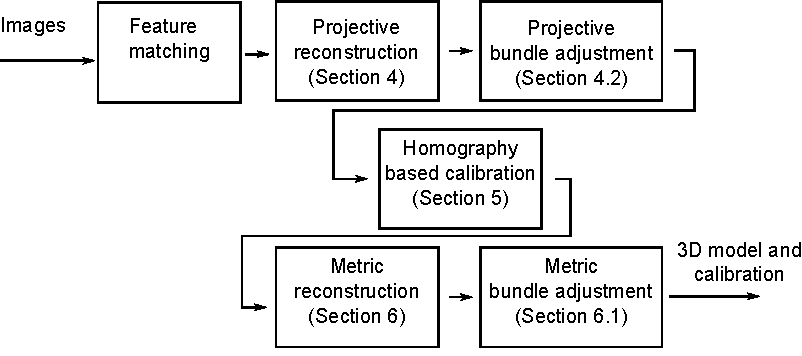
\includegraphics[width=\linewidth]{images/pipeline.pdf}
\caption{The outline of our planar self-calibration algorithm. It first performs a projective reconstruction, then recovers the calibration matrix from the obtained homographies, and then upgrades it to a metric reconstruction.}
\label{fig:diagram}
\end{figure}

\subsection{Paper structure}
asdf

\section{Camera model}

We model our cameras using the well-known pinhole model with radial distortion. The projection function $\pv=\Projection(\xv)$ transforms a point in 3D world space $\xv=[x,y,z]^\top$ to a 2D pixel position $\pv=[u,v]^\top$. The projection function is the composition of four functions: the extrinsic transform $\ExtrinsicFunc$, perspective division $\hnorm$, the distortion function $\Distortion$, and the intrinsic transform $\IntrinsicFunc$, \ie $\Projection(\xv) = \IntrinsicFunc \circ \Distortion \circ \hnorm \circ \ExtrinsicFunc(\xv)$.

The extrinsic transform is a rigid 3D transform that aligns the point with the camera reference frame
%
\begin{align}
\xv_c &= \ExtrinsicFunc(\xv) = \Rm \xv + \tv 
\end{align}
%
where the rotation matrix $\Rm$ and the translation vector $\tv$ are the extrinsic parameters of the camera, \ie its rigid pose. The distorted point $\xv_d$ is obtained by applying the radial distortion function
%
\begin{align}
\xv_d = \Distortion(\xv_n) &= \xv_n (1+r^2 d_0 + r^4 d_1)
\label{eq:distortion}
\end{align}
%
where $r = \norm{\xv_n}$ is the distance to the point from the optical center and the vector $\dv=[d_0,d_1]^\top$ contains the distortion coefficients. Finally, the intrinsic matrix is applied to transform the pixel from metric units to pixel units
%
\begin{align}
\pv &= \IntrinsicFunc(\xv_d) = \hnorm(\Km \homogeneous{\xv}_d)
\\
\Km &= \begin{bmatrix}
f_x & 0 & u_0 \\
0 & f_y & v_0 \\
0 & 0 & 1
\end{bmatrix}
\label{eq:intrinsic_matrix}
\end{align}
%

The camera model contains 6 degrees of freedom (DoF) for the extrinsic parameters (three for rotation and three for translation) and 6 DoF for the intrinsic parameters (two focal lengths, two for the principal point, and two distortion coefficients). 

\subsection{Distortion in pixel space}

It is also possible to model the distortion in pixel space instead of in metric space. This is particularly useful when only a metric reconstruction is not available, as in Section \ref{sec:planar:distortion}. In this case we can define an equivalent projection function $\Projection(\xv) = \Distortion_{\text{px}} \circ \IntrinsicFunc \circ \hnorm \circ \ExtrinsicFunc(\xv)$. This distortion function is defined as
%
\begin{align}
\Distortion_{\text{px}}(\pv) = (\pv - \pv_0)(1+r^2 d'_0 + r^4 d'_1) + \pv_0
\label{eq:distortion_pixels}
\end{align}
%
where $\pv_0$ is the center of distortion and $r=\norm{\pv-\pv_0}$ is the distance of the point from this center. In the common case where the focal lengths of the camera are similar, \ie $f \approx f_x \approx f_y$, the distortion models $\Distortion$ and $\Distortion_{\text{px}}$ are equivalent when $d_0 = f^2 d'_0$, $d_1=f^4 d'_1$, and the center of distortion is the same as the principal point.

\section{Planar self-calibration}
The goal of the calibration algorithm is to recover the intrinsic parameters from a sequence of images of a planar scene. The structure of the method is shown in Figure \ref{fig:diagram}. It has three main stages: projective reconstruction, homography-based calibration, and metric reconstruction. The projective reconstruction calibrates the distortion and produces a set of homographies. The self-calibration algorithm uses these homographies to recover the intrinsic matrix and the pose of the reference camera. Finally, the metric reconstruction optimizes all parameters of the model using all available constraints, thus obtaining the optimal calibration. Each stage contains a closed-form solution and a non-linear optimization of all parameters involved (also known as bundle adjustment)

The following sections describe each stage in detail. The feature matching stage is not described since it can be implemented with any standard feature descriptor and matching approach, \eg \cite{rublee2011orb}.

\subsection{Projective reconstruction}

Planar geometry is well understood and extensively documented. Here we provide a brief review of what is relevant to this paper. Further details can be found in \cite{hartley2000}. We first approach planar geometry using a pinhole camera with no distortion. Section \ref{sec:planar:distortion} addresses the effects of distortion.

A planar scene induces a homography between two pinhole cameras. That is, the measurements of image $a$ are related to those of image $b$ by
%
\begin{align}
\homogeneous{\pv}_b \propto \Hm \homogeneous{\pv}_a 
\label{eq:homography}
\end{align}
%
where $\Hm$ is a $3 \times 3$ full-rank matrix. The equation is up to scale because all elements are in homogeneous coordinates and thus $\Hm$ has only 8 DoF.

The first step in our algorithm is to obtain a projective reconstruction of the scene. The reconstruction includes the position of the observed points in world coordinates and the poses of the cameras. The points can be represented with a 2D position vector $\yv=[x,y]^\top$ because the scene is planar. The poses of the cameras can be represented by a homography that translates the points from world to image space. 

A projective reconstruction is defined up to a homography. Thus, without loss of generality we select a reference frame $r$ to have the same coordinate frame as the world, \ie $\Hm_r = \Im_{3 \times 3}$. This also implicitly fixes the position of the world points $\yv=\pv_r$. The poses of the other frames can be determined independently by computing the homography between them and the reference frame.

\subsubsection{Distortion}
\label{sec:planar:distortion}

The relation of Eq.~\eqref{eq:homography} only holds for a pinhole camera without distortion. We note that in the case of distortion, the undistorted measurements will still follow Eq.~\eqref{eq:homography}. We can thus estimate the distortion model by finding the coefficients that allow the measurements to be modelled by a homography. We use the distortion model from Eq.~\eqref{eq:distortion_pixels} to remove the distortion in image space.

Although there are methods of estimating the distortion parameters from a set of uncalibrated images, we rely on robust homography estimation methods to obtain an initial projective reconstruction assuming no distortion. The distortion coefficients are then estimated during a projective bundle adjustment step. This has proven to work well with moderate distortion levels.

\subsection{Projective bundle adjustment}
\label{sec:projective:ba}

The projective reconstruction obtained so far is biased due to the choice of reference frame and the distortion coefficients haven't been estimated. We perform a robust non-linear minimization \cite{ceres-solver} over all parameters to obtain the optimal projective reconstruction. The formulation of the minimization problem is as follows, 
%
\begin{align}
\argmin_{\dv',\pv_0,\lbrace \Hm_i \rbrace, \lbrace \yv_j \rbrace} 
%
\sum_i \sum_j \rho(\norm{\pv_{ij} - \Distortion_{\text{px}}(\Hm_i \yv_j)})^2 + \norm{\pv_0 - \bar{\pv}_0}
\end{align}
%
where $\rho(\cdot)$ is a robust function to reduce the influence of outliers (\eg the Cauchy loss function \cite{ceres-solver}). The homography of the reference camera is kept fixed to remove the projective ambiguity. However, all point coordinates $\yv_j$ are optimized to remove the bias towards the reference camera. The final term regularizes the center of distortion, biasing it towards the center of the image $\bar{\pv}_0$ in case of no distortion.

\subsection{Homography-based self-calibration}

The calibration constraints come from our knowledge of the metric structure of the world applied to the obtained projective reconstruction. To derive the constraints we arbitrarily choose our metric world coordinate frame to coincide with the camera frame of the reference image. We describe the scene plane in this reference frame by its normal vector $\nv=[n_x,n_y,n_z]^\top$ (with unit norm) and the distance to the origin.

We encode the euclidean structure of the plane with two orthogonal basis vectors with equal norm that span the plane: $\av$ and $\bv$. Like the normal vector, these vectors represent directions in 3D space. Note that these vectors are not unique since we can rotate them around $\nv$ and they are still orthonormal basis vectors. With this in mind, the following equations encode the orthogonality and equal norm constraints respectively
\begin{align}
\av^\top \bv = 0, \label{eq:ortho_constraint_ref} \\
\av^\top \av - \bv^\top \bv = 0. \label{eq:norm_constraint_ref}
\end{align}

We can derive these basis vectors from the plane's normal. To ensure orthogonality, we select $\av$ as the cross product of $\nv$ with an auxiliary fixed vector $\ev$
\begin{align}
\av = \nv \times \ev = [\nv]_\times \ev \\
\bv = \nv \times \av = [\nv]_\times^2 \ev
\end{align}
Note that $\ev$ can be any vector as long as it is not parallel to $\nv$. A different $\ev$ will produce a different orientation for the basis but Equations \eqref{eq:ortho_constraint_ref} and \eqref{eq:norm_constraint_ref} will remain unchanged.

The basis vectors are defined in the coordinate frame of the reference camera. It is possible to transform the basis vectors to the reference frame of camera $i$ through the previously obtained homography
\begin{align}
\av_i = \Km^{-1} \Hm_i \Km \av, \\
\bv_i = \Km^{-1} \Hm_i \Km \bv.
\end{align}
%
We may now enforce the same constraints (orthogonal and equal norm) on the transformed basis vectors
\begin{align}
\av_i^\top \bv_i = 0, \label{eq:ortho_constraint} \\
\av_i^\top \av_i - \bv_i^\top \bv_i = 0. \label{eq:norm_constraint} 
\end{align}
%
Note that Equations \eqref{eq:ortho_constraint_ref} and \eqref{eq:norm_constraint_ref} are satisfied by definition but Equations \eqref{eq:ortho_constraint} and \eqref{eq:norm_constraint} constrain $\Km$ using the reconstructed homographies. These are the self-calibration constraints that will allow us to recover $\Km$.

\subsubsection{Connection with previous work}

Although our derivation takes a different route, the constraints obtained so far are identical to those proposed in \cite{bocquillon2006}. The components of the \emph{circular points} in \cite{bocquillon2006} $\xv_1$ and $\xv_2$ are simply the images of the basis vectors (\ie $\xv_1=\Km \av$ and $\xv_2=\Km \bv$). Equations \eqref{eq:ortho_constraint} and \eqref{eq:norm_constraint} can be expanded to be expressed as in \cite{bocquillon2006}
%
\begin{align}
\av_i^\top \bv_i &= (\Km^{-1} \Hm_i \Km \av)^\top (\Km^{-1} \Hm_i \Km \bv) \notag \\
&= (\Km^{-1} \Hm_i \xv_1)^\top (\Km^{-1} \Hm_i \xv_2) \notag \\
&= \xv_1^\top \Hm_i^\top \omegav \Hm_i \xv_2 = 0 
\\
\av_i^\top \av_i - \bv_i^\top \bv_i &= (\Km^{-1} \Hm_i \Km \av)^\top (\Km^{-1} \Hm_i \Km \av) \notag 
\\
&\quad - (\Km^{-1} \Hm_i \Km \bv)^\top (\Km^{-1} \Hm_i \Km \bv) \notag 
\\
&= (\Km^{-1} \Hm_i \xv_1)^\top (\Km^{-1} \Hm_i \xv_1) \notag 
\\
&\quad - (\Km^{-1} \Hm_i \xv_2)^\top (\Km^{-1} \Hm_i \xv_1) \notag 
\\
&= \xv_1^\top \Hm_i^\top \omegav \Hm_i \xv_1 - \xv_2^\top \Hm_i^\top \omegav \Hm_i \xv_2 = 0 
\end{align}
which are the exact same constraints and with the same parametrization as in Equation (4) of \cite{bocquillon2006}. The resulting unknowns are $\Km$ and $\nv$. The normal $\nv$ has 3 variables with 2 DoF. The intrinsic matrix $\Km$ varies between 5 DoF and 1 DoF depending on the camera model. $\ev$ is not an unknown of the problem. It can be chosen arbitrarily and fixed as long as it is not parallel to the normal vector.

\subsubsection{Scale and normalization}

The self-calibration constraints are homogeneous in the absence of noise. In this case their scale does not matter. However, with real data the constraints will have non-zero residuals and their scale affects the solution obtained. For example, Eq.~\eqref{eq:ortho_constraint} can also be expressed as
\begin{align}
\av_i^\top \bv_i = \norm{\av_i} \norm{\bv_i} \cos \theta_{a b}
\end{align} 
where $\theta$ is the angle between the vectors. We see that the scale of the residuals is directly proportional to the norm of the vectors. However, this constraint should only depend on the angle because it is an orthogonality constraint. Similarly, Eq.~\eqref{eq:norm_constraint} should only constrain the norms of the vectors to be equal regardless of their scale.

It is important to note that the homographies themselves are defined up to scale and may produce very different norms for $\av_i$ and $\bv_i$. Moreover the norm of basis vectors also depends on the angle between the chosen $\ev$ and the estimated normal which may vary during optimization. The Equations as presented in the previous section might bias the solution towards a certain plane normal or give more weight to certain homographies to compensate for large differences in scale between residuals. Therefore we propose a normalized pair of constraints that is scale independent 
\begin{align}
\frac{\av_i' \cdot \bv_i'}{\norm{\av_i} \norm{\bv_i}} = 0 \label{eq:ortho_constraint_normalized}\\
1 - \frac{\norm{\bv_i}^2}{\norm{\av_i}^2} = 0 \label{eq:norm_constraint_normalized}
\end{align}
These are the normalized planar self-calibration constraints.

\subsubsection{Closed-form with a known plane normal}

The normalized constraints can be readily used in an iterative non-linear minimization procedure to find the optimum values for the intrinsic parameters and the normal vector. However, we need an initial guess that we'd like to obtain in closed-form. A closed-form solution can be easily obtained if we assume a known plane normal and a simplified camera model. 

We reduce the intrinsic matrix to have 1 DoF by assuming a single focal length and a known principal point. We use the distortion center obtained in Sec.~\ref{sec:projective:ba} as the principal point and translate the obtained homographies so that this point lies in the origin. The intrinsic matrix is then $\Km=\text{diag}(f, f, 0)$. We use the original constraints \eqref{eq:ortho_constraint} and \eqref{eq:norm_constraint} to avoid the non-linearities introduced by the normalization.

To fix the plane normal we assume that the reference image was taken perpendicular to the plane, \ie $\nv=[0,0,1]^\top$. This is a strong assumption, however it is only used to obtain an initial guess of the focal length. Moreover, different initial guesses for the focal length can be obtained very cheaply by selecting the different input images as reference images. The best initial guess from these can then be used for further optimization. The experiments presented in Section \ref{sec:results} explore the sensitivity of the algorithm to this assumption.

Under these assumptions the constraints \eqref{eq:ortho_constraint} and \eqref{eq:norm_constraint} reduce to a series of quadratic polynomials in one variable 
\begin{align}
h_{31}\, h_{32}\, f^2 + h_{11}\, h_{12} + h_{21}\, h_{22}=0
\label{eq:closed_form_a}
\\
f^2\, {h_{31}}^2 - f^2\, {h_{32}}^2 + {h_{11}}^2 + {h_{21}}^2 - {h_{12}}^2 - {h_{22}}^2=0
\label{eq:closed_form_b}
\end{align}
Note that since $\nv$ is known the choice of $\ev$ vanishes. Choosing either $\ev=[1,0,0]^\top$ or $\ev=[0,1,0]^\top$ result in the same equations. However, choosing $\ev=[0,0,1]^\top$ (\ie $\ev=\nv$) results in the trivial constraint $0=0$.

\subsubsection{Minimal configuration}

According to \cite{hartley2000} the problem of planar calibration is well constrained when $2m \geq v+4$ where $m$ is the number of views and $v$ is the DoF of the intrinsic parameters. However, \cite{hartley2000} used 4 DoF for the circular points. The current formulation makes these a function of the normal vector and thus reduces them to 2 DoF. Thus, the minimal configuration requires $2m \geq v+2$. For example, if we only want to estimate the focal length ($2m \geq 1+2$) one homography is enough, as demonstrated by Eqs.~\eqref{eq:closed_form_a} and \eqref{eq:closed_form_b}.

\subsubsection{Non-linear optimization}

The closed-form solution provides an initial guess under the fixed-normal assumption. Although rough, this is a suitable starting point for a non-linear optimization using the constraints \eqref{eq:ortho_constraint_normalized} and \eqref{eq:norm_constraint_normalized}. The formulation of the minimization problem is as follows, 
%
\begin{align}
\argmin_{\Km,\nv} 
\sum_i 
\frac{\av_i \cdot \bv_i}{\norm{\av_i} \norm{\bv_i}} +
\sum_i 
1 - \frac{\norm{\bv_i}^2}{\norm{\av_i}^2}
\end{align}
%
where the normal vector is constrained to have unit norm and $\Km$ is allowed to have 4 DoF as in \eqref{eq:intrinsic_matrix}. We note that although this non-linear minimization is necessary to improve the initial guess, it is still not optimal because the camera poses is encoded into the homographies and cannot be optimized. The optimal solution will be obtained by optimizing in metric space.

\subsection{Metric reconstruction}

Once the intrinsic parameters have been recovered, upgrading the projective reconstruction to a metric reconstruction is straightforward. We define a new world reference frame so that the scene's plane lies at $z=0$. Under this reference frame, the extrinsic parameters of the reference camera are $\Rm=[\av, \bv, \nv]^\top$ and $\tv= - \Rm \nv$, which positions the camera exactly one unit away from the plane center and aligns it with the recovered normal.

The position $\xv$ of the observed points can be obtained by intersecting the optical ray of the reference camera with the scene plane at $z=0$. The extrinsic parameters of the other cameras is implicitly contained in the homographies and could be directly recovered from them using non-linear means. Alternatively, since the observed points are already triangulated and the camera is calibrated we can use well-known perspective-n-points techniques to estimate the extrinsics \cite{pnp}.

This produces a complete and calibrated 3D reconstruction of the scene and the cameras, including the intrinsic parameters ($\Km,\dv$), the extrinsic parameters ($\lbrace \Rm_i \rbrace,\lbrace \tv_i \rbrace$), and the point 3D positions ($\lbrace \xv_j \rbrace$).

\subsection{Metric bundle adjustment}

The final solution is obtained by a non-linear optimization in metric space. This implicitly enforces all known constraints about the scene and uses all available information. The formulation of the minimization problem is as follows, 
%
\begin{align}
\argmin_{\Km,\dv,\lbrace \Rm_i \rbrace,\lbrace \tv_i \rbrace, \lbrace \xv_j \rbrace} 
%
\sum_i \sum_j \rho(\norm{\pv_{ij} - \Projection_i(\xv_j))})^2 
\end{align}
%
where the position of the points is constrained so that $z=0$. 

\section{Experimental results}
\label{sec:results}

- Synthetic tests, error in calibration with increasing noise in point position (compared to bouguet and ground truth). See Fig.~\ref{fig:synth_results}.

- Error in calibration with increasing angle to plane normal for reference image (shows robustness to main assumption)

- Synthetic tests, error without scale normalization of residuals (shows why we are better than \cite{bocquillon2006}). Don't know if this will work.

- Practical calibrations of real cameras (comapred to bouguet, no ground truth)

- Augmented reality of a plane (images + video)

\begin{figure}
\centering
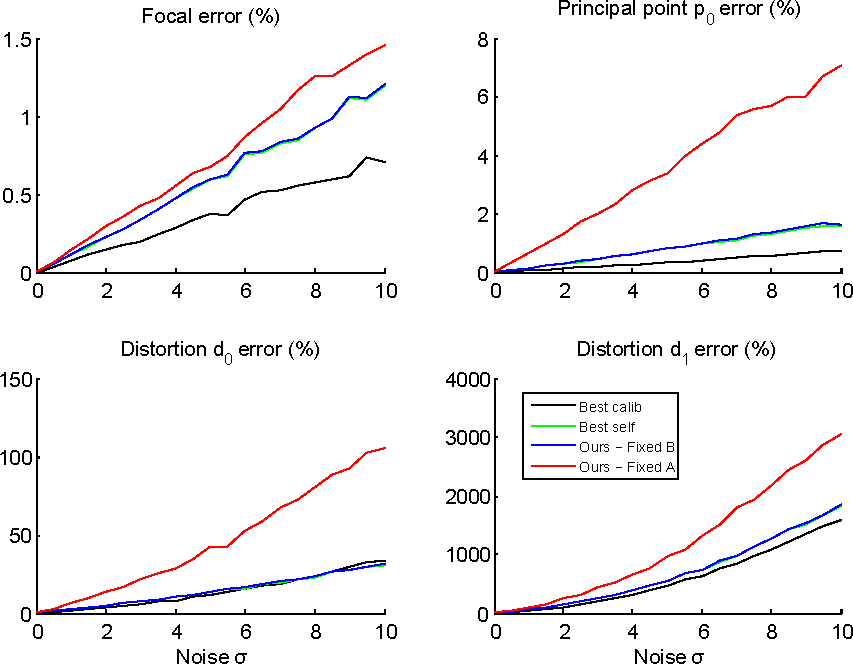
\includegraphics[width=\linewidth]{images/resultsPointNoise.pdf}
\caption{Synthetic tests results. Error in the intrinsic parameters under noisy point correspondences. y-axis is median over 50 experiments. x-axis is the $\sigma$ of gaussian noise applied to the point correspondences. Blue: all cameras pointing at the center of the scene. Green: rotated and translated cameras. Red: using ground truth for 3D point position (\cite{zhang1999}).}
\label{fig:synth_results}
\end{figure}

\begin{figure}
\centering
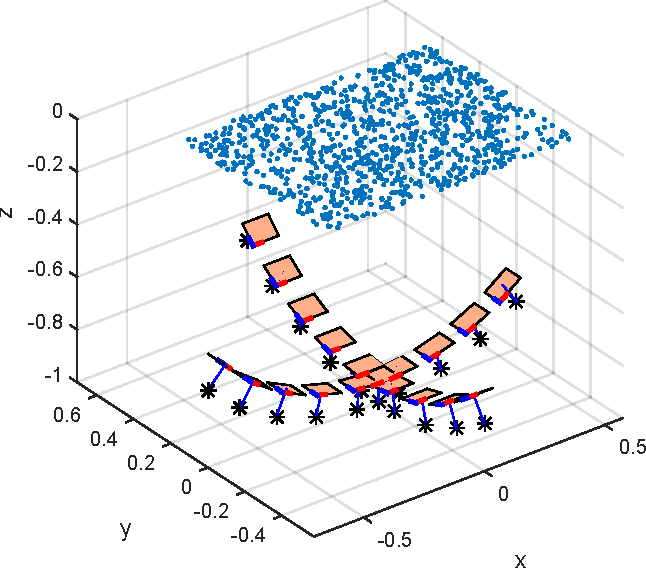
\includegraphics[width=0.45\linewidth]{images/synthCameraPosesRotation.pdf}
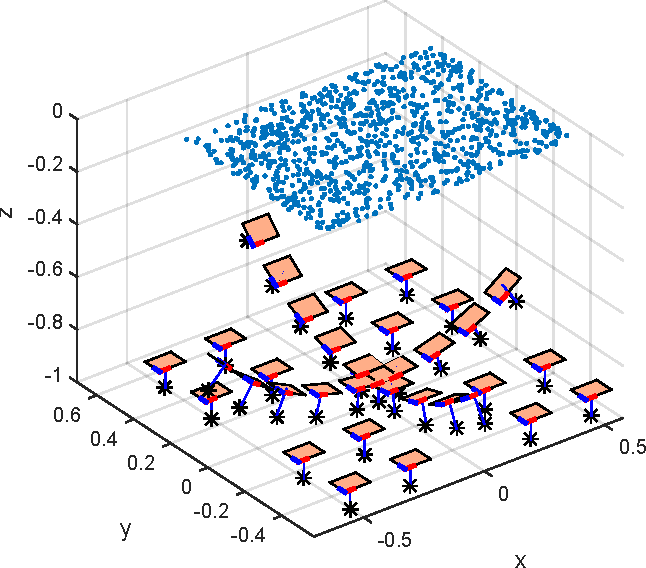
\includegraphics[width=0.45\linewidth]{images/synthCameraPosesTranslation.pdf}
\caption{Synthetically generated scenes used for testing.}
\label{fig:synth_poses}
\end{figure}

\section{Conclusions}

{\small
\bibliographystyle{ieee}
\bibliography{planecalib_paper}
}

\end{document}
